\documentclass[11pt]{article}
\usepackage[italian]{babel}
\usepackage[utf8]{inputenc}	% Para caracteres en español
\usepackage{amsmath,amsthm,amsfonts,amssymb,amscd}
\usepackage{multirow,booktabs}
\usepackage[table]{xcolor}
\usepackage{fullpage}
\usepackage{lastpage}
\usepackage{enumitem}
\usepackage{fancyhdr}
\usepackage{mathrsfs}
\usepackage{wrapfig}
\usepackage{graphicx}
\graphicspath{ {./images/} }
\usepackage{setspace}
\usepackage{calc}
\usepackage{multicol}
\usepackage{cancel}
\usepackage[retainorgcmds]{IEEEtrantools}
\usepackage[margin=3cm]{geometry}
\usepackage{amsmath}
\newlength{\tabcont}
\setlength{\parindent}{0.0in}
\setlength{\parskip}{0.05in}
\usepackage{empheq}
\usepackage{framed}
\usepackage[most]{tcolorbox}
\usepackage{xcolor}
\usepackage{FiraSans}
\usepackage{listings}
\usepackage{color} %red, green, blue, yellow, cyan, magenta, black, white
\definecolor{mygreen}{RGB}{28,172,0} % color values Red, Green, Blue
\definecolor{mylilas}{RGB}{170,55,241}
\colorlet{shadecolor}{orange!15}
\parindent 0in
\parskip 12pt
\geometry{margin=1in, headsep=0.25in}
\theoremstyle{definition}
\newtheorem{defn}{Definizione}
\newtheorem{reg}{Regola}
\newtheorem{oss}{Osservazione}
\newtheorem{exer}{Esecizio}
\newtheorem{note}{Nota}
\newtheorem{thm}{Teorema}[section] % reset theorem numbering for each chapter
\theoremstyle{plain}
\newcommand{\restr}[2]{%
\mathchoice{%
\restriction{#1}{#2}{\displaystyle}%
}{%
\restriction{#1}{#2}{\textstyle}%
}{%
\restriction{#1}{#2}{\scriptstyle}%
}{%
\restriction{#1}{#2}{\scriptscriptstyle}%
}%
}

\lstset{language=Matlab,%
    %basicstyle=\color{red},
    breaklines=true,%
    morekeywords={matlab2tikz},
    keywordstyle=\color{blue},%
    morekeywords=[2]{1}, keywordstyle=[2]{\color{black}},
    identifierstyle=\color{black},%
    stringstyle=\color{mylilas},
    commentstyle=\color{mygreen},%
    showstringspaces=false,%without this there will be a symbol in the places where there is a space
    numbers=left,%
    numberstyle={\tiny \color{black}},% size of the numbers
    numbersep=9pt, % this defines how far the numbers are from the text
    emph=[1]{for,end,break},emphstyle=[1]\color{red}, %some words to emphasise
    %emph=[2]{word1,word2}, emphstyle=[2]{style},    
}


\newlength{\totbarheight}
\newlength{\bardepth}




\begin{document}

\title{Interpolazione Polinomiale}
\author{Guglielmo Bartelloni}
\maketitle

\thispagestyle{empty}

\begin{center}
{\LARGE \bf 23 Marzo 2022}\\
\end{center}

Noi sappiamo che:
\[
||e||\le a(1+\varDelta_n)w(f_i;\frac{b-a}{n})
.\] 

Supponiamo di scegliere una partizione dell'intervallo [a,b]:
\[
	\varDelta={a=x_0<x_1<...<x_n=b}
.\] 
Quindi consideriamo n sottointervalli, $[x_{i-1},x_{i}]$ $i=1,...,n$ tale che, detta: $h=max(x_{i},x_{i-1})\to 0 \ \ \ \ n\to \infty$
e supponiamo che in ciascuno sottointervallo la f(x) sia interpolata da un polinomio di grado n \textbf{fissato} (quindi interpolo ogni sottoinrevallo).

Ottengo quindi una funzione \textbf{polinomiale a tratti}, chiamiamola $s_m$, tale che, detto $e(x)=s_m(x)-f(x)$ si avra:
\[
	||e||\le a(1+\varDelta_m)w(f;h)\to 0\ quando\ h\to 0 \implies\ n\to \infty
.\] 

\begin{defn}
	Assegnato la partizione $\varDelta={a=x_0<x_1<...<x_n=b}$ diremo che $s_m$ e' una \textbf{spline di grado n} sulla partizione $\varDelta$ se:
	\begin{enumerate}
		\item $sm_{\mkern 1mu \vrule height 2ex\mkern2mu [x_{i-1},x_i]} (x)\in \Pi_m$
		\item $S_m \in C^{m-1}[a,b]$ $\to$  (derivabile m-1 volte e continua)
	\end{enumerate}
\end{defn}
\begin{oss}
	Il requisito 2) significa richiedere che (la derivata j-esima):
	\[
		sm^{j}_{\mkern 1mu \vrule height 2ex\mkern2mu [x_{i-1},x_i]}(x_{i})=sm^{j}_{\mkern 1mu \vrule height 2ex\mkern2mu [x_{i},x_{i+1}]}(x_{i})
	.\] 
con $i=1,...,n-1$ e $j=0,...,m-1$

Quindi nel punto $x_{i}$ le derivate devono essere uguali
\end{oss}

\begin{oss}
	\begin{enumerate}
		\item Se $s_m$ fosse un polinomio allora sarebbe una spline
		\item Se $\alpha$,$\beta\in R$, $s_m$ $g_m\in S_m(\varDelta)$: su $\varDelta$
			\[
				\alpha S_m(x)+Bg_m(x)\in S_m(\varDelta)
			.\] 
		Sono anch'essi spline e pertanto $S_m(\varDelta)$ e' \textbf{uno spazio vettoriale}
	\end{enumerate}
\end{oss}
\begin{thm}
	$dim(S_m(\varDelta)=m+n)$, pertanto sono necessarie n+m condizioni indipendenti per individuare univocamente una spline interpolante di grado m su una partizione $\varDelta$
\end{thm}
\begin{defn}
	Una spline di grado m sulla partizione $\varDelta$ $S_m(x)$, si dice \textbf{interpolante una funzione} $f(x)$ se:
	\[
		s_m(x_{i})=f_i=f(x_{i})\ \ \ i=0,...,n
	.\] 
\end{defn}
\begin{oss}
	Le condizioni di interpolazione sono n+1, pertanto esse permettono di individuare univocamente solo una spline di grado 1 o lineare (n+m dove m=1) ovvero la spezzata congungente i punti $(x_{i},f_i)$ $i=0,...,n$. La sua espressione e' data da:
	\[
		s1_{\mkern 1mu \vrule height 2ex\mkern2mu [x_{i-1},x_i]}(x)=\frac{(x_{i}-x_{i-1})f_i+(x_{i}-x)f_{i-1}}{x_{i}-x_{i-1}}\ \ \ per\ \ \ i=1,...,n
	.\] 

\section{Spline Cubiche}
	$s_3(x)$ sara tale che: \[
		s3_{\mkern 1mu \vrule height 2ex\mkern2mu [x_{i-1},x_i]}(x)\le \Pi_3,\ s_3(x)\in C^{2}[a,b]
	.\] 
Per individuare in maniera univoca si ha bisogno di \textbf{n+3} condizioni.

Le condizioni di interpolazione sono n+1 quindi ci mancano due condizioni. Vediamo quindi alcuni modi di interpolare: ciascuno di essi dara origine ad una spline cubica interpolante \textbf{diversa}
	\subsection{Spline Cubica Naturale}
	$s_3''(a)=0$ e $s_3''(b)=0$
	\subsection{Spline Cubica Completa}
	$s_3'(a)=f'(a)$ e $s_3'(b)=f'(b)$
	\subsection{Spline Cubica Periodica}
	Si applica nel caso in cui $f(x)$ sia periodica e l'intervallo [a,b] contenga m numero intero di periodi (es.1) imponendo le condizioni.
	$s_3'(a)=s_3'(b)$ e $s_3''(a)=s_3''(b)$
	\subsection{Spline not-a-knot (implementato da matlab spline())}
	In questo caso si richiede che le restrizioni di $s_3(x)$ sugli intervalli $[x_0,x_1]$ e $[x_1,x_2]$ siano lo \textbf{stesso polinomio}, si richiede che le restrizioni di $s_3(x)$ sugli intervalli $[x_{n-2},x_{n-1}]$ e $[x_{n-1},x_n]$ siano lo stesso polinomio.

	Ragioniamo su $[x_0,x_1]$ e $[x_1,x_2]$. Supponiamo che $s_3(x)\in C^{2}[a,b]$, pertanto: 
	\[
		s3^{j}_{\mkern 1mu \vrule height 2ex\mkern2mu [x_{0},x_1]}(x_1)=s3^{j}_{\mkern 1mu \vrule height 2ex\mkern2mu [x_{1},x_2]}(x_1)\ \ \ \ j=0,1,2
	.\] 
se imponiamo che la $s3^{j}_{\mkern 1mu \vrule height 2ex\mkern2mu [x_{0},x_1]}(x_1)=s3^{j}_{\mkern 1mu \vrule height 2ex\mkern2mu [x_{1},x_2]}(x_2)$ allora i \textbf{due polinomi coincideranno} (perche 4 ingonite).

Questo imopone che \[
	\frac{s_3^{2}(x_1)-s_3^{2}(x_0)}{x_1-x_0}=\frac{s_3^{2}(x_2)-s_3^{2}(x_1)}{x_2-x_1}
.\] 

Simmetricamente si richiedera per gli ultrimi 2 sottointervalli che:
\[
	\frac{s_3^{2}(x_{n-1})-s_3^{2}(x_{n-2})}{x_{n-1}-x_{n-2}}=\frac{s_3^{2}(x_n)-s_3^{2}(x_{n-1})}{x_n-x_{n-1}}
.\] 


\end{oss}

\begin{center}
{\LARGE \bf 24 Marzo 2022}\\
{\large Calcolo Numerico}\\
\end{center}

\section{Calcolo Spline Cubiche naturali}

Oggi vediamo come si calcano le spline cubiche naturali.
Le spline cubiche non hanno il problema del malcondizionamento crescente, al crescere di n, e si puo dimostrare che, se $f \in C^{(4)}[a,b]$:
 

\[
	||f^{(j)}-s_{3}^{(j)}||=O(h^{4-j})
.\] 
Per $j=0,1,2$

Questo vale per tutte le spline cubiche viste, tranne quella naturaleche ha un piccolo errore agli estremi dell'intervallo (per le condizioni imposte), tuttavia, si smezza esponenzialmente agli estremi dell'intervallo. Pertanto abbiamo necessita di definire un algoritmo efficiente per il calcolo di $s_3(x)$. Esamineremo in dettaglio il calcolo di una spline cubica naturale anche se gli argomenti si possono generalizzare alle spline cubiche di altro tipo (sul libro not-a-knot).

Preliminarmente diamo il seguente risultato:

\begin{thm}
$\forall m\ge 2$: se $s_m$ e' una spline di grado m su $\varDelta$, allora $s_m$ e' una spline di grado m-1 su $\varDelta$
\end{thm}

\begin{proof}
Immediata dalla definizione di spline di grado m su $\varDelta$.
\end{proof}

\section{Calcolo di una spline cubica naturale} 
($s_3''(a)=s_3''(x_0)=0$, $s_3''(b)=s_3''(x_n)=0$)

Se $s_3(x)$ e' una spline cubica su $\varDelta$ allora la $s_3'(x)$ e' una spline quadratica su $\varDelta$ (per il teorema sopra) e, quindi, $s_3''(x)$ e' una spline lineare su $\varDelta$.

\[
	s_3(x)\ cubica\to s_3'(x)\ quadratica\to s_3''(x)\ lineare
.\] 

Supponiamo di conoscere i valori di $f_i=f(x_i)$ per i=0,..,n della funzione interpolante.

Poiche $s_3''(x)$ e' una spline lineare, detta $m_i=s_3''(x)$ per i=0,...,n si avra:


\[
	f_{\mkern 1mu \vrule height 2ex\mkern2mu [x_{i-1},x_i]}(x)=\frac{(x-x_{i-1})^{2}m_i-(x_{i}-x)^{2}m_{i-1}}{2h_i}+q_i\ i=1,...,n
.\] 
(2)

in cui $q_i$ e' una costante di integrazione

Integrando ancora la (2), otteniamo:
\[
	s3_{\mkern 1mu \vrule height 2ex\mkern2mu [x_{i-1},x_i]}(x)=\frac{(x-x_{i-1})^{3}m_i+(x_{i}-x)^{3}m_{i-1}}{6h_i}+q_i(x-x_{i-1})+r_i\ i=1,...,n
.\] 

Dove $r_i$ e' una nuova costante di integrazione. Imponendo le condizioni di interpolazione in $x_{i-1}$ e $x_{i}$, si ottiene:
\[
	s3_{\mkern 1mu \vrule height 2ex\mkern2mu [x_{i-1},x_i]}(x_{i-1})=\frac{h_i^{2}}{6}m_{i-1}+r_i=f_{i-1}
.\] 
Faccio la formula inversa
\[
	r_i=f_{i-1}-\frac{h_{i-1}^{2}}{6}m_{i-1}
.\] 

\[
	s3_{\mkern 1mu \vrule height 2ex\mkern2mu [x_{i-1},x_i]}(x_{i})=\frac{h_i^{2}}{6}m_{i}+q_ih_i+r_i=f_{i}
.\] 
\[
	h_iq_i=f_i-f_{i-1}+\frac{h_i^{2}}{6}m_i
.\] 

\[
h_iq_i=f_i-f_{i-1}+\frac{h_i^{2}}{6}m_{i-1}-\frac{h_i^{2}}{6}m_{i}
.\] 

\[
	q_i=\frac{f_i-f_{i-1}}{h_i}-\frac{h_i}{6}(m_i-m_{i-1})
.\] 
La prima frazione del secondo membro e' una differenza divisisa in particolare $f[x_{i-1},x_{i}]$

Pertanto potremo calcolare la spline cubica in ogni sottointervallo a patto di calcolare $m_i$ per $i=1,...,n-1$ ($m_0=m_n=0$). Per calcolare questi valori essendo $s_3'(x)$ una spline qudratica su $\varDelta$, imponendo che:
\[
	s3'_{\mkern 1mu \vrule height 2ex\mkern2mu [x_{i-1},x_i]}(x_{i})=s3'_{\mkern 1mu \vrule height 2ex\mkern2mu [x_{i},x_{i+1}]}(x_{i})\ per\ i=1,...,n-1
.\] 

Quindi abbiamo un sistema di n-1 equazioni in n-1 incognite, esplicitiamolo:
\[
\frac{h_i}{2}m_i+q_i=-.\frac{h_{i+1}}{2}m_i+q_{i+1}
.\] 
Raccolgo il tutto
\[
\frac{h_i+h_{i+1}}{2}m_i=q_{i+1}-q_i
.\] 
\[
	=f[x_{i},x_{i+1}]-f[x_{i-1},x_{i}]-\frac{h_{i+1}}{6}(m_{i+1}-m_i)+\frac{h_i}{6}(m_i-m_{i+1})
.\] 
moltiplico per 6 e porto al primo membro tutto quello che non e' una differenza divisa
\[
	3(h_i+h_{i+1})m_i+h_{i+1}m_{i+1}+h_im_{i-1}=6(f[x_{i},x_{i+1}]-f[x_{i-1},x_{i}])
.\] 
Divido membro a mebro per $h_i-h_{i+1}$
\[
	\frac{h_i}{h_i+h_{i+1}}m_{i+1}+2m_{i}+\frac{h_{i+1}}{h_i+h_{i+1}}m_{i+1}=6 \frac{f[x_{i},x_{i+1}]-f[x_{i-1},x_{i}]}{h_i+h_{i+1}}
.\] 
Ponendo
\[
q_i=\frac{h_i}{h_i+h_{i+1}}\ \ \ \ \psi_i=\frac{h_{i+1}}{h_i+h_{i+1}}
.\] 

E osservando che 
\[
	\frac{f[x_{i},x_{i+1}]-f[x_{i-1},x_{i}]}{h_i+h_{i+1}}=f[x_{i-1},x_{i},x_{i+1}]
.\] 
dove $h_i+h_{i+1}=x_{i+1}-x_{i-1}$

Si ottiene che il sistema lineare tridiagonale

\[
	q_im_{i-1}+2m_i+\psi_im_{i+1}=6f[x_{i-1},x_{i},x_{i+1}]\ \ \ i=1,...,n-1
.\] 

In forma vettoriale, si ottiene, ricodando che $m_0=0\ e\ m_n=0$:

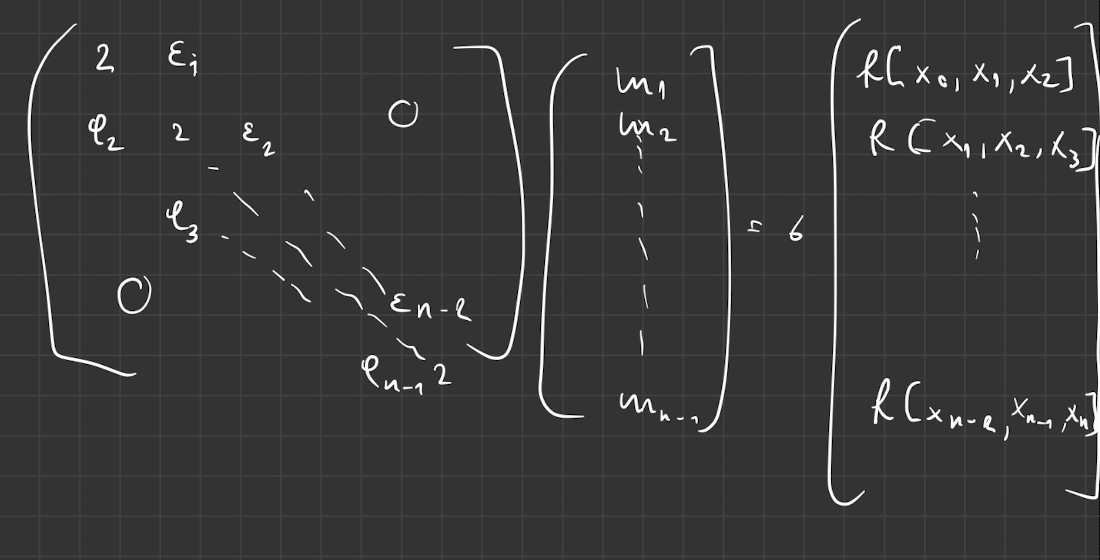
\includegraphics[width=\textwidth]{matrice_lu_spline_cubica}

Osserviamo che $q_i\ e\ \psi_i>0$ per $\forall i=1,...,n$
Inoltre
\[
q_i+\psi_i=1
.\] 
Pertanto la matrice dei coefficienti e' diagonale dominante per righe. Pertanto la sua fattorizzazione LU e' sempre definita (inoltre si puo vedere essere sempre ben condizionata, indipendentemente dalla sua dimensione). Andiamo a vedre come si possa risolvere con complessita lineare.

Infatti, sono necessari, in tutto 4 vettori:

Uno che contiene in ingresso il termine noto e puo essere riscritto con la soluzione del sistema lineare.
Tre che contengono in ingresso gli elementi sulle 3 diagonali dei fattori L e U che al pari della matrice, sono sparsi

\begin{center}
{\LARGE \bf 30 Marzo 2022}\\
{\large Calcolo Numerico}\\
\end{center}

\section{Risoluzione del sistema lineare della spline cubica naturale}
Il sistema lineare della lezione precedente e' \textbf{sparso}, nel senso che molti degli elementi della matrice dei coefficienti sono null. (In generale per una matrice sparsa il numero di elementi non nulli e' \textbf{lineare} nella dimensione, invece che essere una frazione del quadrato).

Questa matrice si puo fattorizzare con un costo lineare.

Motivati da quanto sopra, andiamo a definire un algoritmo di fattorizzazione LU efficiente per una \textbf{generica matrice tridiagonale}.

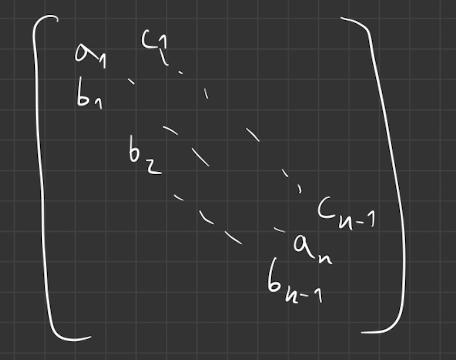
\includegraphics[width=\textwidth]{matrice_da_risolvere}

\begin{oss}
	Pertanto, per memorizzare la matrice $T_n$ saranno sufficienti 3 vettori di lunghezza n,
	Definiamo a, b e c, tali che:
	\begin{itemize}
		\item $a_i$ = i-esimo elemento della diagonale principlae,
		\item $c_i$ = i-esimo elemento della sopradiagonale,
		\item $b_i$ = i-esimo elemento della sottodiagonale
	\end{itemize}

\end{oss}

Verifichiamo che $T_n=L_nU_n$ , 

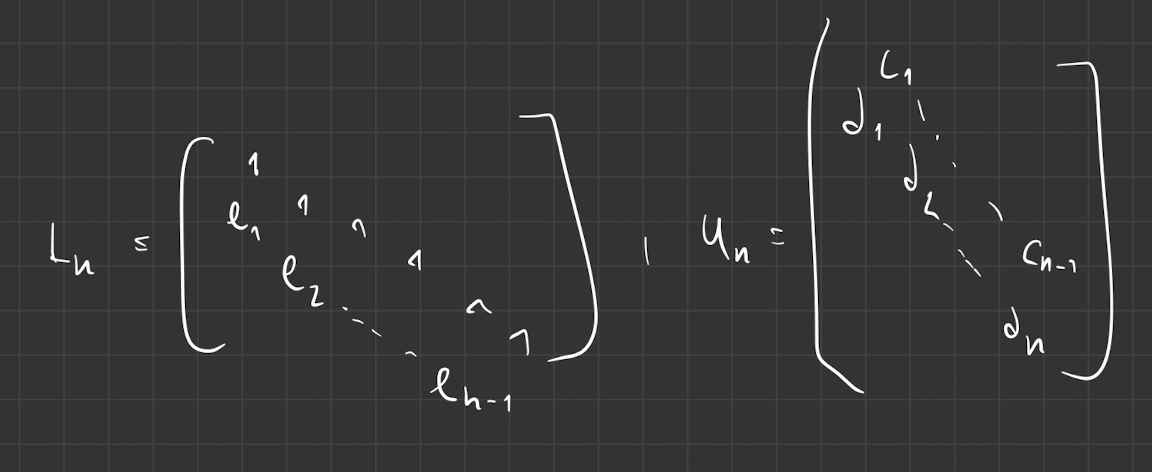
\includegraphics[width=\textwidth]{matrici_l_n}

con $l_i=\frac{b_i}{d_{i}}$ , $d_{i+1}=a_{i+1}-l_{i}c_{i}$  per $i=1,...,n-1$ e $d_1=a_1$ 

Verifichiamo questo facendo il prodotto $L_nU_n$  ed uguagliando gli elementi omomloghi:

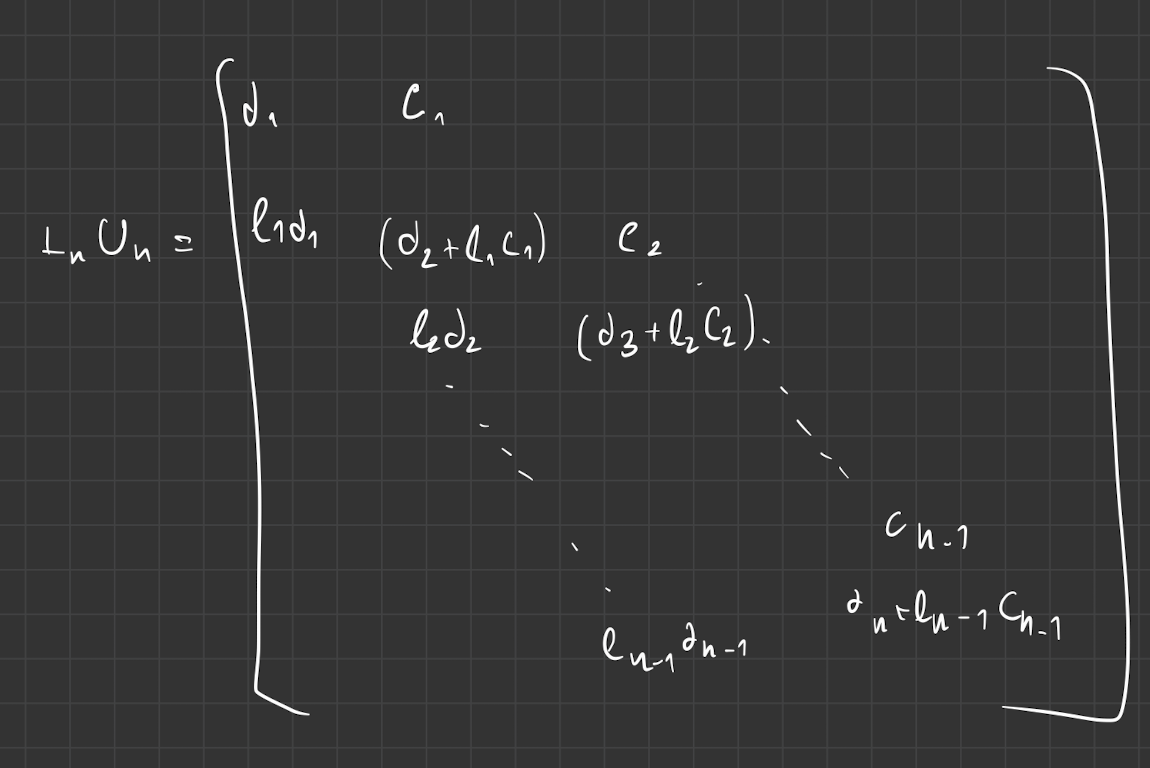
\includegraphics[width=\textwidth]{matrice_tn}

$d_1=a_1$, $d_{i+1}+l_{i}c_{i}=a_{i+1}$ , $i=1,...,n-1$ e $l_{i}d_{i}=b_{i}$ 

Pertanto:
\[
d_1=a_1
.\] 
\[
l_{i}=\frac{b_{i}}{d_{i}}
.\] 
\[
b_{i+1}=a_{i+1}-l_{i}c_{i},\ \ \ i=1,...,n-1
.\] 

Costo totale: $3(n-1)$ flops.

Se utilizziamo questa fattorizzazione per risolvere.


$T_nx=f=[f_1,...,f_n]^{T}$ 

Allora dobbiamo risolvere $L_ny=f$ e, quindi $U_nx=y$. Nella pratica, lo stesso vettore che contiene il termine noto puo essere sovrascritto con i vettori y e x.
(Possiamo sovrascrivere i tre vettori iniziali con i tre vettori di cui sopra)

\[
L_ny=f\Leftrightarrow y_1=f_1
.\] 

\begin{lstlisting}
for i=1:n-1
\end{lstlisting}

	$y_{i+1}=f_{i+1}-l_{i}y_{i}$ 

\begin{lstlisting}
end
\end{lstlisting}

Questo da luogo ad 2(n-1) flops

\[
U_nx=y \Leftrightarrow x_n= \frac{y_n}{d_n}
.\] 

\begin{lstlisting}
for i=n-1:-1:1
\end{lstlisting}

	$x_{i}=\frac{f_{i}-c_{i}x_{i+1}}{d_{i}}$ 

\begin{lstlisting}
end
\end{lstlisting}

Questo costa 3(n-1) flops.

In tutto il costo e' di 8n flops quindi un costo lineare.

Su moodle c'e' un'implementazione efficiente dell'algoritmo di risoluzione di un sistema tridiagonale.
\end{document}
